% THIS IS SIGPROC-SP.TEX - VERSION 3.1
% WORKS WITH V3.2SP OF ACM_PROC_ARTICLE-SP.CLS
% APRIL 2009

\documentclass{acm_proc_article-sp}

\usepackage[slovene,english]{babel}
\usepackage[utf8]{inputenc}

\begin{document}

\title{FbHash: shema za izračun podobnosti datotek v digitalni forenziki}
%\title{FbHash: A New Similarity Hashing Scheme for Digital Forensics}
%TODO naslov v slovenščini, recimo "FbHash: shema za izračun podobnosti datotek v digitalni forenziki" ali "FbHash: shema za detekcijo podobnih datotek v digitalni forenziki"
%\subtitle{[Extended Abstract]
%\titlenote{A full version of this paper is available as
%\textit{Author's Guide to Preparing ACM SIG Proceedings Using
%\LaTeX$2_\epsilon$\ and BibTeX} at
%\texttt{www.acm.org/eaddress.htm}}}

\numberofauthors{3} 
\author{
\alignauthor
Timotej Knez \\
Fakulteta za računalništvo in informatiko \\
Univerza v Ljubljani%
%63160163%\titlenote{Dr.~Trovato insisted his name be first.}\\
%       \affaddr{Institute for Clarity in Documentation}\\
%       \affaddr{1932 Wallamaloo Lane}\\
%       \affaddr{Wallamaloo, New Zealand}\\
%       \email{trovato@corporation.com}
% 2nd. author
\alignauthor
Sebastian Mežnar\\
Fakulteta za matematiko in fiziko \\
Univerza v Ljubljani%
%27192031 %\titlenote{The secretary disavows
%any knowledge of this author's actions.}\\
%       \affaddr{Institute for Clarity in Documentation}\\
%       \affaddr{P.O. Box 1212}\\
%       \affaddr{Dublin, Ohio 43017-6221}\\
%       \email{webmaster@marysville-ohio.com}
% 3rd. author
\alignauthor 
Jasmina Pegan \\
Fakulteta za računalništvo in informatiko \\
Univerza v Ljubljani%
%63170423%\titlenote{This author is the
%one who did all the really hard work.}\\
%       \affaddr{The Th{\o}rv{\"a}ld Group}\\
%       \affaddr{1 Th{\o}rv{\"a}ld Circle}\\
%       \affaddr{Hekla, Iceland}\\
%       \email{larst@affiliation.org}
}

\date{20. maj 2020}

\maketitle
\begin{abstract}
Algoritmi za detekcijo podobnih datotek pomagajo digitalnim forenzikom pri obdelavi velikih količin podatkov. V delu predstavimo algoritem za detekcijo podobnih datotek \texttt{FbHash}, opisan v članku~\cite{fbhash} in nekaj njegovih predhodnikov. Predstavimo in implementiramo tudi svojo različico algoritma \texttt{FbHash}. Implementacijo testiramo na istih množicah datotek kot avtorji članka ter predstavimo naše ugotovitve.
Rezultati eksperimentov se ujemajo z rezultati v članku, saj naša implementacija algoritma doseže F-score 94\%.
\end{abstract}

\category{E.3}{Data encryption}{}

\terms{Zgoščevanje} % hashing

\keywords{prstni odtis datoteke, podobnostni izvleček, zabrisano zgoščevanje, TF-IDF, kosinusna podobnost}
%Data fingerprinting, Similarity digests, Fuzzy hashing, TF-IDF, Cosine-similarity} 
\section{Uvod}
Živimo v obdobju shranjevanja ogromnih količin podatkov. Pri forenzičnih preiskavah se pogosto zgodi, da je pridobljenih datotek preveč za ročno pregledovanje. Digitalni forenziki se tako soočijo s problemom avtomatizacije preiskave datotek. Možna rešitev so algoritmi za detekcijo podobnih datotek (angl. \emph{Approximate Matching algorithms}), kot so \texttt{ssdeep}, \texttt{sdhash} in \texttt{FbHash}, ki poskusijo filtrirati vnaprej znane "slabe" oziroma "dobre" datoteke. Ti algoritmi ugotavljajo delež ujemanja datotek s pomočjo (nekriptografskih) zgoščevalnih funkcij. Algoritma \texttt{ssdeep} in \texttt{sdhash} lahko preslepi aktivni napadalec, ki pametno napravi majhne spremembe na določenih mestih datoteke. Učinkovitega napada na algoritem \texttt{FbHash} ne poznamo~\cite{fbhash}.
%TODO
% nekej o FbHash-B in S in primeri tipa datotek
% še kaj o naši implementaciji, poskusih, rezultatih
\\
\subsection{Prispevek \v{c}lanka}

V našem delu predstavimo članek \cite{fbhash}, v katerem avtorji predstavijo zgoščevalno funkcijo \texttt{FbHash}, ki omogoča lažje filtriranje "dobrih" in "slabih" datotek pri preiskovanju. 

Glavni prispevki raziskave v \cite{fbhash} so:
\begin{itemize}
  \item Predstavijo shemo za približno ujemanje, ki je odporno proti aktivnemu napadalcu.
  \item Predstavijo algoritma za zgoščevanje stisnjenih in nestisnjenih datotek, ki temeljita na shemi TF-IDF \cite{Ramos_usingtf-idf}.
  \item Podajo analizo algoritma \texttt{FbHash} z drugimi algoritmi, ki rešujejo isti problem.
  \item Prikažejo, da iskanje podobnosti na nivoju zlogov ni dovolj pri stisnjenih datotekah.
  \item Naredijo analizo varnosti za \texttt{FbHash} in pokažejo, da je varen proti napadom z aktivnim napadalcem.
\end{itemize}

Poleg tega v našem delu algoritem ponovno implementiramo in preizkusimo različne variante funkcij za uteževanje, ki se pojavijo v algoritmu. Rezultati naše implementacije algoritma se ujemajo z rezultati v~\cite{fbhash}. Algoritem vedno zazna podobnost v datotekah z vsaj $5\%$ ujemanja. Ugotovimo tudi, da za dobre rezultate zadošča relativno majhna baza datotek.

\subsection{Struktura članka}

Naš članek je organiziran na sledeč način. V 2. poglavju predstavimo predhodnike algoritma \texttt{FbHash}. V 3. poglavju podrobneje predstavimo algoritem \texttt{FbHash} in našo implementacijo. V 4. poglavju povzamemo ugotovitve v delu~\cite{fbhash}. V 5. poglavju opišemo izvedene eksperimente, v 6. pa predstavimo njihove rezultate. Narejeno delo povzamemo in zaključimo v 7. poglavju.

\section{Sorodna dela}
Prvi algoritem namenjen iskanju približnih ujemanj je bil objavljen leta 2002 pod imenom \texttt{dcfldd}. Ta algoritem je razvil N. Harbour kot izboljšano verzijo ukaza \texttt{dd}~\cite{dcfldd}. Izboljšana različica tega algoritma je \texttt{ssdeep}. Pomembnejša predhodnika algoritma \texttt{FbHash} sta tudi \texttt{MRSH-v2} in \texttt{mvHash-B}. Obstaja še \texttt{bbhash}, ki pa je časovno potraten in ga ne bomo podrobneje opisali.

\subsection{ssdeep}
Algoritem \texttt{ssdeep} je implementacija kontekstno sprožene kosovno zgoščevalne funkcije (angl. \emph{Context Triggered Piecewise Hash}, CTPH), ki jo je predstavil J. Kornblum septembra 2006 v raziskavi~\cite{kornblum:ctph}. Algoritem temelji na detektorju neželene elektronske pošte \texttt{spamsum}, ki lahko zazna sporočila, ki so podobna znanim neželenim sporočilom.

CTPH uporablja zgoščevanje po kosih (angl. \emph{piecewise hashing}), kar pomeni, da se zgoščena vrednost izračuna na posameznih delih datoteke fiksne dolžine. Za razliko od \texttt{dcfldd} algoritem CTPH uporabi poljubno zgoščevalno funkcijo.

Drugi princip, ki ga uporablja CTPH, je zgoščevalna funkcija z drsečim oknom (angl. \emph{rolling hash}), ki preslika zadnjih $k$ zlogov v psevdonaključno vrednost. Vsakega naslednika je tako možno hitro izračunati iz predhodno izračunane vrednosti. Pri tem je uporabljena zgoščevalna funkcija \texttt{FNV}.

Postopek CTPH se začne z izračunom zgoščenih vrednosti z drsečim oknom. Ob določeni sprožilni zgoščeni vrednosti (angl. \emph{trigger value}) se vzporedno s tem sproži še algoritem zgoščevanja po kosih. Ob ponovni pojavitvi sprožilne vrednosti se dotlej zbrane vrednosti druge zgoščevalne funkcije zapišejo v končni prstni odtis.
Tako se ob lokalni spremembi v datoteki sprememba pozna le lokalno tudi v prstnem odtisu.

Sledi primerjava prstnih odtisov datotek, ki temelji na uteženi Levenstheinovi razdalji (angl. \emph{edit distance}), ki je nato še skalirana in obrnjena, da predstavlja $0$ povsem različna prstna odtisa, $1$ pa povsem enaka.

Algoritem \texttt{ssdeep}, ki je implementacija CTPH, se izkaže pri primerjavi podobnih besedilnih datotek in dokumentov~\cite{kornblum:ctph}. Po drugi strani pa lahko aktivni napadalec popravi "slabe" datoteke na tak način, da se izognejo črni listi~\cite{fbhash}. Ker je prstni odtis fiksne dolžine, je algoritem primeren le za relativno majhne datoteke podobnih velikosti.

\subsection{sdhash}
Algoritem \texttt{sdhash} je opisal V. Roussev januarja 2010 v delu~\cite{roussev:sdhash}. Glavna prednost tega algoritma pred predhodnimi je, da izbere statistično manj verjetne dele datotek kot izhodišče za računanje prstnega odtisa.

Postopek se začne z iskanjem statistično najmanj verjetnih delov datoteke. Izračuna se entropija skupin po $k$ zlogov datoteke. Nato se izračuna rank vsake skupine glede na $n$ sosednjih skupin. Izbrane so skupine, ki imajo rank večji ali enak postavljeni meji.

Sledi filtriranje skupin $k$ zlogov, ki niso bistvene, povzročajo pa lažno pozitivne rezultate. Ocenili so, da je dobro zavreči skupine z oceno entropije pod $100$ ali nad $990$, ker so takšne skupine pogoste npr. v datotekah tipa JPEG.

Nato se generira prstni odtis datoteke kot zaporedje Bloomovih filtrov, ki so verjetnostni bitni vektorji, uporabljeni za prostorsko učinkovito predstavitev množic. Bloomov filter, ki predstavlja prazno množico, je vektor samih ničel. Ko dodamo element v tako predstavljeno množico, vzamemo fiksno število zgoščenih vrednosti elementa. Zgoščene vrednosti so definirane tako, da element preslikajo v pozicijo v vektorju. Nato dobljene pozicije v vektorju nastavimo na $1$. Na sliki~\ref{bloom} vidimo, kako lahko preverimo, ali je nek element v Bloomovem filtru. Z več zgoščevalnimi funkcijami določimo pozicije v bitnem vektorju, ki morajo vse biti enake $1$. Vidimo, da so $x$, $y$ in $z$ elementi filtra, $w$ pa ne.
\begin{figure}
\centering
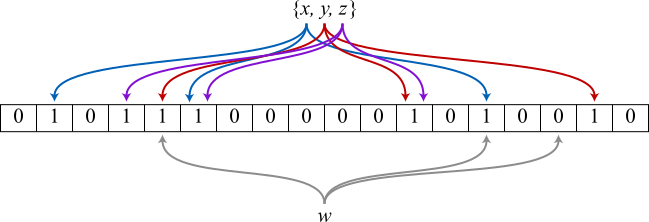
\includegraphics[width=\linewidth]{bloom.png}
\caption{Prikaz preverjanja, ali je element v Bloomovem filtru. Element $w$ ni v filtru, ker zadnja zgoščevalna funkcija ne kaže na enico.}
\label{bloom}
\end{figure}
Algoritem \texttt{sdhash} preveri za vsako izbrano skupino $k$ zlogov, ali je že v množici, predstavljeni z Bloomovimi filtri. Če skupine ni v množici, jo algoritem doda.

Nazadnje algoritem primerja prstne odtise datotek, torej zaporedje Bloomovih filtrov. Za vsak filter, ki predstavlja prvo datoteko, se izračuna maksimalna ocena podobnosti s filtri, ki predstavljajo drugo datoteko. Rezultat je povprečje tako pridobljenih ocen podobnosti.

Algoritem \texttt{sdhash} doseže boljša priklic in preciznost kot \texttt{ssdeep}~\cite{fbhash}. A tudi ta algoritem ima več pomanjkljivosti: nekaterih datoteke ne more primerjati, primerjava datoteke same s seboj lahko vrne oceno med $50$ in $100$ ter prvih $15$ zlogov sploh ne vpliva na končni prstni odtis. Poleg naštetega aktivni napadalec lahko spremeni "slabe" datoteke na tak način, da se izognejo črni listi oziroma "dobre" datoteke tako, da se obdržijo na beli listi~\cite{breitinger2012security}.

\subsection{MRSH-v2}
Oktobra 2012 sta F. Breitinger in H. Baier predstavila algoritem \texttt{MRSH-v2}~\cite{mrsh-v2}, ki se opira na predhodno razvit algoritem \texttt{MRSH} (angl. \emph{multi-resolution similarity hashing}), ta pa temelji na algoritmu \texttt{ssdeep}. 

Algoritem \texttt{MRSH} ima določene sprožilne točke $(-1)\,mod\,b$, kjer $b$ pomeni povprečno velikost bloka. Namesto zgoščevalne funkcije z drsečim oknom uporabi polinomsko zgoščevalno funkcijo \texttt{djb2}, kot primitiv pa \texttt{MD5}. Namesto konkatenacije zgoščenih vrednosti \texttt{MRSH} kot prstni odtis uporabi seznam Bloomovih filtrov. 

Algoritem \texttt{MRSH-v2} ponovno uporabi zgoščevalno funkcijo z drsečim oknom, kot \texttt{ssdeep}, namesto \texttt{FNV} pa uporabi funkcijo zgoščevanja \texttt{MD5}. Za večjo hitrost in v izogib napadu z dodajanjem sprožilnih točk je dodana tudi spodnja meja za velikost skupin zlogov $\frac{b}{4}$. 

Algoritem \texttt{MRSH-v2} je po~\cite{mrsh-v2} časovno učinkovitejši od predhodnih algoritmov. Vključuje način za odkrivanje fragmentov in način za odkrivanje podobnih datotek. Po analizi leta 2014~\cite{breitinger2014}, ki primerja \texttt{ssdeep}, \texttt{sdhash} in \texttt{MRSH-v2}, se v povprečju najbolje obnese \texttt{sdhash}, \texttt{ssdeep} in \texttt{sdhash} izkazujeta dobro preciznost, vsi trije algoritmi pa imajo relativno slab priklic.

\subsection{mvHash-B}
Marca 2013 so F. Breitinger in sod. predstavili algoritem \texttt{mvHash-B}~\cite{mvhash-b}. Ideja algoritma je, da majhne lokalne spremembe ne spremenijo končnega rezultata. 

V prvem koraku se izvede večinsko glasovanje po bitih z nastavljivo mejo $t$. Vsakih $k$ zlogov se tako preslika v ničle, če je število enic v zaporedju bitov manjše od $t$, sicer pa v enice.

Nato se zaporedje bitov zapiše na bolj kompakten način -- enake zaporedne bite nadomestimo z dolžino takega niza. Če se zaporedje bitov ne začne z nekaj ničlami, bo prvo število v seznamu 0. Dobimo kodirano zaporedje dolžin nizov.

Kodirano zaporedje se razdeli v prekrivajoče se skupine fiksne dolžine. Te skupine so dodane v Bloomov filter.
Nazadnje se primerja Bloomove filtre s pomočjo Hammingove razdalje, ocene pa se povpreči in odšteje od $100$. 

Algoritem \texttt{mvHash-B} naj bi bil hiter skoraj kot \texttt{SHA-1}, torej blizu zgornje meje učinkovitosti~\cite{mvhash-b}. Vendar tudi ta algoritem ni varen pred aktivnim napadalcem, saj je možno popraviti "slabo" datoteko tako, da se izogne črni listi~\cite{chang2016security}.

\section{Opis algoritma}

Avtorji v članku~\cite{fbhash} predstavijo algoritem \texttt{FbHash-B}, ki je namenjen nestisnjenim (angl. \emph{uncompressed}) in \texttt{FbHash-S}, ki je namenjen stisnjenim (angl. \emph{compressed}) datotekam. Iskanje želenih datotek poteka na sledeč način. Najprej datoteke, ki jih želimo preveriti zgostimo s pomočjo ustreznega algoritma glede na njihov tip in tako dobim bazo podatkov. Nato zgostimo še ciljne datoteke in jih primerjamo z datotekami iz baze podatkov. Tako lahko datoteke, ki imajo s ciljnimi dovolj podobnosti zavržemo (angl. \emph{whitelist}) oziroma dodamo med iskane (angl. \emph{blacklist}).
%[jasmina] js tle bolj razumem da črna lista so iskane datoteke (known-to-be-bad)
%Tako lahko datoteke, ki imajo s ciljnimi dovolj podobnosti zavržemo (ang. blacklist) oziroma dodamo med iskane (angl. \emph{whitelist}).

\subsection{FbHash-B}

\texttt{FbHash-B} je bolj primeren za datoteke, ki niso stisnjene. V opisu algoritma bomo za boljšo preglednost uporabili sledečo notacijo:
% TODO: mogoce zmanjsaj prostor med dvema tockama
\begin{itemize}
  \item Del datoteke: niz $k$ zaporednih zlogov. 
  \item $ch_{i}^D$: del datoteke $D$, ki se začne na $i$-tem zlogu.
  \item Frekvenca dela oziroma $chf_{ch_i}^D$: število pojavitev dela datoteke $ch_i$ v datoteki $D$.
  \item Datotečna frekvenca dela oziroma $df_{ch}$: število datotek, ki vsebujejo del datoteke $ch$.
  \item $N$: število datotek v bazi podatkov.
  \item $RollingHash(ch_i)$: vrednost rekurzivne zgoščevalne funk-cije imenovane rolling hash na delu datoteke $ch_i$
  \item $chw_{ch_i}^D$: utež dela datoteke $ch_i$ v datoteki $D$
  \item $docw_{ch_i}$: datotečna utež dela datoteke $ch_i$
  \item $W_{ch_i}^D$: ocena dela datoteke $ch_i$ v datoteki $D$
\end{itemize}

Algoritem bomo predstavili v treh delih. V prvem delu datoteko razdelimo v dele, ki jih zgostimo z zgostitveno funkcijo in pretvorimo v utež glede na število njihovih pojavitev v datoteki. V drugem delu izračunamo datotečne uteži glede na to, v koliko datotekah se zgostitev dela pojavi. V tretjem delu pa iz datotečnih uteži in uteži dela izračunamo zgostitveno oceno, ki predstavlja datoteko.

\subsubsection{Računanje frekvence delov datotek}

V tem koraku se izračunajo frekvence delov datotek in njihove uteži. Vsaka datoteka vsebuje $N_D - k$ delov datotek, kjer je $N_D$ dolžina datoteke $D$ v zlogih in $k$ parameter. Tako ima $i$-ti del datoteke $D$ obliko $B_{i}^{D}B_{i+1}^{D} \cdots B_{i+k-1}^{D} = ch_{i}^D$, kjer je $B_{j}^{D}$ $j$-ti zlog datoteke $D$.

Najprej izračunamo $RollingHash(ch_{0}^D)$ s formulo: 
\[RollingHash(ch_{0}^D) = B_{0}^{D} \cdot a^{k-1} + \cdots + B_{k-1}^{D} \cdot a^0 \pmod n,\]
kjer so $a$, $n$ in $k$ parametri. Zaradi rekurzivne strukture funkcije $RollingHash$ lahko zgostitve preostalih delov izračunamo na sledeč način:
\begin{align*}
Rolling&Hash(ch_{i+1}^D) = \\
&a \cdot RollingHash(ch_{i}^D)-B_{i}^{D} \cdot a^{k}-B_{i+k}^D \pmod n.
\end{align*}

Parametre $a$, $k$ in $n$ izberemo na sledeč način. Za $a$ izberemo neko konstanto med $2$ in $255$. Če za zalogo vrednosti funkcije RollingHash vzamemo $64$-bitna števila, lahko $k$ izračunamo na sledeč način: \begin{displaymath}  B_{i}^{D} \cdot a^{k-1} \leq 2^{64}-1.\end{displaymath} Ker je maksimalna vrednost zloga in parametra $a$ enaka $255$ dobimo neenačbo $255^k \leq 2^{64}-1$ iz česar sledi, da je $k$ manjši ali enak $7$. Tako za $k$ izberemo $7$. Če želimo zagotoviti, da ne pride do trkov med različnimi deli datotek, moramo za $n$ izbrati praštevilo, ki je večje od $2^{56}=255\cdot 255^{k-1}$. 

Strukturo datoteke lahko tako predstavimo kot razpršeno tabelo, kjer je kjuč vrednost, ki jo dobimo s funkcijo $RollingHash$ na določenem delu datoteke, vrednost pa število pojavitev pripadajočega dela datoteke (oziroma vrednosti, ki smo jo dobili s funkcijo $RollingHash$).

Prvi korak zaključimo tako, da izračunamo uteži za dele besedila znotraj datoteke ($chw_{ch_i}^D$) s pomočjo ene izmed funkcij iz~\ref{weight-functions}. 

\subsubsection{Računanje datotečnih uteži}

Drugi korak je računanje datotečnih uteži delov besedila. Te nakazujejo koliko informacije prinese posamezen del datoteke znotraj določene baze podatkov. 

Najprej je potrebno izračunati datotečno frekvenco za dele datotek, ki se v bazi podatkov pojavijo. To naredimo tako, da zgradimo razpršeno tabelo katere ključ je vrednost \\ $RollingHash(ch_i)$, vrednost pa število pojavitev posameznega ključa. To s tabelo lahko sestavimo tako, da se sprehodimo čez vse ključe razpršenih tabel za posamezni datoteke in zgoščevalni tabeli prištejemo $1$, če se ključ v datoteki pojavi.

Iz frekvence posameznega dela nato izračunamo njegovo datotečno utež ($docw_{ch_i}$) s pomočjo ene izmed funkcij iz~\ref{weight-functions}.

\subsubsection{Računanje zgostitvenih ocen}

V tretjem koraku izračunamo zgostitvene ocene za posamezne datoteke. S temi ocenami lahko kasneje datoteke med seboj primerjamo, kot je predstavljeno v~\ref{doc-compare}.

V vsaki datoteki izračunamo oceno posameznega dela datoteke s formulo: \begin{displaymath}  W_{ch_i}^D = docw_{ch_i} \cdot chw_{ch_i}^D. \end{displaymath}

Zgostitveno oceno za datoteko predstavimo kot razpršeno tabelo, kjer za ključ vzamemo vrednosti funkcije $RollingHash$, ki smo jih dobili v datoteki, vrednosti pa so ocene dela datoteke ($W_{ch_i}^D$).

\subsection{FbHash-S}

Med testiranjem različnih datotek so avtorji dela ugotovili, da algoritem \texttt{FbHash-B} na stisnjenih datotekah (tipov docx, pptx, pdf, zip ...) ne deluje najbolje. Tako datoteki, ki imata $90$\% podobnost v datoteki tipa docx, nimata veliko podobnosti na nivoju zlogov. Zato so razvili tudi verzijo algoritma \texttt{FbHash-S}, ki dosega dobre rezultate tudi na stisnjenih datotekah.

Algoritem \texttt{FbHash-S} deluje na sledeč način. Najprej datoteko razširimo (angl. \emph{uncompress}) in uporabimo algoritem \texttt{FbHash-B} na vsaki izmed dobljenih datotek. Končna ocena pomembnosti je izračunana kot povprečje ocen posameznih datotek.

Zaradi dodatnega dela je algoritem \texttt{FbHash-S} časovno bolj zahteven od algoritma \texttt{FbHash-B}.

\subsection{Primerjanje datotek}
\label{doc-compare}

Podobnost med datotekama izračunamo s pomočjo kosinusne razdalje~\cite{Salton88term-weightingapproaches}. Najprej poskrbimo, da ima vsaka izmed datotek izračunano tabelo ocen pomembnosti. Podobnost med datotekama tako izračunamo s formulo: \begin{displaymath} Similarity(D_1, D_2)=\frac{\sum_{i=0}^{n-1} W_{ch_i}^{D_1} \cdot W_{ch_i}^{D_2}}{\sqrt{\sum_{i=0}^{n-1} (W_{ch_i}^{D_1})^2}\cdot\sqrt{\sum_{i=0}^{n-1} (W_{ch_i}^{D_2})^2}}\cdot 100. \end{displaymath} Pri implementaciji lahko opazimo, da lahko za vsako datoteko vnaprej izračunamo $\sum_{i=0}^{n-1} W_{ch_i}^{D}$ in da je v števcu dovolj, da zmnožimo ocene pomembnosti, ki so v preseku ključev.

\subsection{Uporabljene funkcije za uteževanje}
\label{weight-functions}

Tukaj bomo predstavili različne funkcije, ki smo jih preizkusili za iskanje primernih uteži posameznih delov datoteke. Prve se uporabljajo za računanje uteži posameznega dela datoteke, druge pa za računanje datotečne uteži dela datoteke.

\subsubsection{Funkcije za računanje uteži dela besedila}\label{utezivclanku}
Najprej si oglejmo funkcijo za računanje uteži dela besedila, ki je predstavljena v delu~\cite{fbhash}:
\[ W_{ch_i}^{D}(ch f_{ch}^D) = 1 + \log_{10}\left(\frac{ch f_{ch}^D}{N^D}\right),\]
pri čemer $N^D$ predstavlja število delov v datoteki, ki poskrbi za normalizacijo števila delov. Bolj kot je kos datoteke pogost, višja je njegova utež. Relativna frekvenca dela besedila je število med $0$ in $1$, torej je njegov logaritem med $-\infty$ in $1$, saj je $\log_{10}(0)$ enak $-\infty$, $\log_{10}(1)$ pa 0. Menimo, da je to napaka (ali pa so avtorji članka uporabili drugačno funkcijo normiranja kot mi, saj je nikjer ne opišejo), poleg tega pa v delu omenjata \textit{TF-IDF} shemo, katera za izračun uteži pogosto uporabi formulo
\begin{displaymath}\log\left(1 + \frac{ch f_{ch}^D}{N^D}\right).\end{displaymath}
Zato smo uteži dela besedila izračunali nekoliko drugače.

Funkcijo smo popravili, da je rezultat število na intervalu med $0$ in $1$. Izračunamo relativno frekvenco dela in za $1$ povečan rezultat logaritmiramo:
\[ W_{ch_i}^{D}(ch f_{ch}^D) = \log_2\left(1 + \frac{ch f_{ch_i}^D}{N^D}\right). \]
Ker je ulomek povečan za $1$ število na intervalu $[1, 2]$, smo vzeli logaritem z bazo $2$. Tako kot utež dobimo število med $0$ in $1$. 

Predlagamo še drugo funkcijo za računanje uteži, ki je razmerje med frekvenco dela besedila in številom takih delov besedila $n$. Tako je rezultat na intervalu $[0,1]$:
\[ W_{ch_i}^{D}(ch f_{ch}^D) = \frac{ch f_{ch_i}^D}{N^D}. \]

\subsubsection{Funkcije za računanje datotečnih uteži}
Prvo verzijo funkcije za izračun datotečne uteži dela besedila smo povzeli po raziskavi v~\cite{fbhash}. Raziskava poda datotečno utež kot logaritmirano relativno frekvenco datotek, ki vsebujejo posamezen kos $ch_i$:
\[ docw_{ch_i}^{D}(df_{ch}) = \log_{10}\left(\frac{N}{df_{ch}}\right). \]
Notranji ulomek je število med $1$ in $N$, torej je rezultat število med $0$ in $\log_{10}(N)$. Bolj kot je kos datoteke pogost, manjšo utež dobi.

Predlagamo še drugo verzijo funkcije za računanje datotečne uteži. Ulomek obrnemo in odštejemo od $1$, da dobimo vrednost na intervalu $[0, 1]$, ki je še vedno obratno sorazmerna pogostosti dela datoteke:
\[ docw_{ch_i}^{D}(df_{ch}) = 1 - \log_{10}\left(1+\frac{df_{ch}}{N}\right).\]

\section{Ugotovitve \v{c}lanka}

Avtorji v delu svoj algoritem testiranjo in pokažejo, da je varen proti aktivnemu napadalcu.

\subsection{Varnost proti aktivnemu napadalcu}

Napad z aktivnim napadalcem je napad, ko ima napadalec možnost spreminjanja datoteke. Varnost algoritma je prikazana tako, da opišemo znane napade na algoritme iskanja približnih ujemanj in podamo argumente, zakaj tak napad na \texttt{FbHash} ne deluje.

V članku~\cite{5931110} opišejo naslednji napad na \texttt{ssdeep}~\cite{kornblum:ctph}, ki datoteke spremeni tako, da se prikažejo, čeprav so na "črni listi". \texttt{Ssdeep} datoteko razdeli na 64 delov, ki jih zgosti s pomočjo kriptografske funkcije (naprimer md5). Tako je nastali podpis dolg 64 zlogov. Podpis datoteke na "črni listi" se ujema s podpisom datoteke, če se v njem ujema vsaj podniz dolg 7 zlogov. Želja napadalca je, da podpis povsem spremeni s čim manj spremembami v datoteki. To lahko naredi tako, da spremeni datoteko na način, da se vsak sedmi zlog spremeni ali pa vstavi delčke, ki zagotovijo, da se bo datoteka delila na različnih mestih in imela posledično različen podpis. Ta napad na algoritem \texttt{FbHash} ne deluje, saj se ob majhni spremembi datoteke frekvenca delov datoteke le malo spremeni.

V delu~\cite{breitinger2012security} prikažejo, da se lahko oceno podobnosti algoritma \texttt{sdhash} zlahka zniža pod 28\%. Algoritem \texttt{sdhash} je razbit tudi v raziskavi v~\cite{chang2015collision}, ki pokaže, da lahko zgradimo več različnih datotek, katerih podobnost z podano datoteko bo enaka 100\%. Ta napada sta možna zato, ker je končna ocena sestavljena le iz dela datoteke. V \texttt{FbHash} je končna ocena sestavljena iz celotne datoteke, zato je vsaka sprememba opazna in ne prevelika.

Chang v delu~\cite{chang2016security} prikaže, da lahko napadalec algoritem \texttt{mvhash-v} prelisiči in dobi nizko oceno podobnosti z drugo datoteko tudi ko sta datoteki zelo podobni. To je možno zato, ker \texttt{mvhash-v} uporabi funkcijo, ki podatke zgosti. \texttt{FbHash} zgostitvene funkcije ne uporabi, zato je na tak napad odporen.

\subsection{Testiranje algoritma}
% TODO opisi so mogoce malo cudni
Algoritem \texttt{FbHash} je v članku primerjan z algoritmoma \texttt{ssdeep} in \texttt{sdhash}. Njegovo delovanje je primerjano po dveh metrikah: detekcija fragmentov in korelacija skupnega dela datoteke. Detekcija fragmentov nam pove, kako dobro algoritem zazna, da del datoteke (fragment) spada k določeni datoteki. Korelacija skupnega dela datoteke pa nam pove, kako dobro algoritem zazna, da dve datoteki vsebujeta enak del.

\subsubsection{Detekcija fragmentov}

Testi detekcije fragmentov so bili narejeni na bazi podatkov, ki je sestavljena iz fragmentov različnih velikosti in vzetih iz različnih mest v datoteki. Pri tem so uporabljene tekstovne datoteke in datoteke tipa docx iz \cite{zdataset}.

Rezultati, ki jih avtorji dobijo na tekstovnih podatkih so prikazani na sliki~\ref{fig:fd-rez}. X-os grafa prikazuje velikost fragmenta, stolpci povprečno oceno podobnosti med delom in datoteko, točke povezane z daljicami pa prikazujejo procent pravilne korelacije dela z datoteko med poskusi. Vidimo lahko, da so rezultati algoritma \texttt{ssdeep} najslabši in da ocena podobnosti zelo pade, ko je fragment manjši od 50\%. Za \texttt{sdhash} je opazno, da je ocena podobnosti skoraj v vseh primerih najvišja, a da pravilnost korelacije zelo pade, ko je del manjši od 15\%. \texttt{FbHash} v vseh poskusih zazna, da sta del in datoteka korelirana, a je povprečna ocena podobnosti manjša od ocene algoritma \texttt{sdhash}.  

\begin{figure}[htb]
\begin{center}
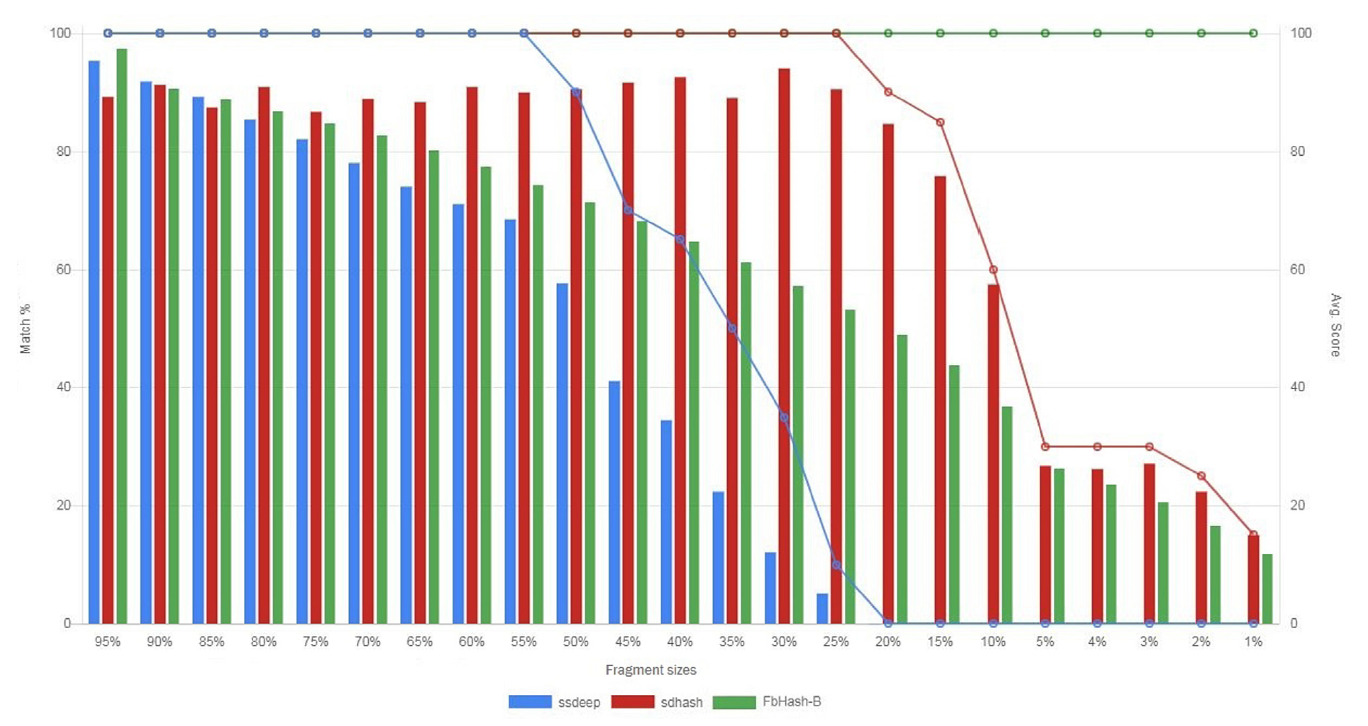
\includegraphics[width=1\columnwidth]{frag_det_text.png}
\end{center}
\caption{\small{Rezultati testiranja avtorjev na tekstovnih datotekah. Vir: \cite{fbhash}}}
\label{fig:fd-rez}
\end{figure}

Poleg tega preverijo natačnost algoritmov z metriko  \texttt{F-score}, katere formula je:
\begin{displaymath} F-score = 2\cdot\frac{precision\cdot recall}{precision + recall},\end{displaymath} 
kjer sta vrednosti precision in recall izračunani s formulama
\begin{displaymath} precision = \frac{TP}{TP + FP},\quad recall = \frac{TP}{TP+FN}.\end{displaymath} 
Tukaj TP predstavlja pravilno pozitiven primer, FP napačno pozitiven primer in FN napačno negativen primer. Na tekstovnih datotekah se je \texttt{FbHash} v vseh testih z metriko F-score izkazal najbolje, saj je imel rezultat med 94\% in 98\%. \texttt{Sdhash} in \texttt{ssdeep} pa sta imela rezultat 89,5\% in 69\%.

Rezultati testiranja na datotekah tipa docx so vidni na sliki~\ref{fig:fd-docx-rez}. Vidimo lahko, da je tako kot na tekstovnih datotekah tudi tukaj \texttt{ssdeep} v obeh kategorijah najslabši in da ima  \texttt{sdhash} višjo povprečno oceno kot algoritem \texttt{FbHash-B}, a del datoteke pravilno korelira z datoteko v manj primerih. \texttt{Sdhash} ima tukaj pri vsaki velikosti fragmenta podobno oceno (okoli 10\%) in verjetnost korelacije (okoli 24\%). Podobno je mogoče opaziti tudi v algoritmu \texttt{FbHash-B}, katerega ocena se giblje okoli 9\% in verjetnost korelacije okoli 100\%. Tako verjetnost korelacije ima v vseh primerih tudi algoritem \texttt{FbHash-S}, ki je bil narejen prav za datoteke tega tipa. To je vidno pri povprečni oceni, ki je pri vseh velikostih občutno višja od ocene drugih algoritmov.

\begin{figure}[htb]
\begin{center}
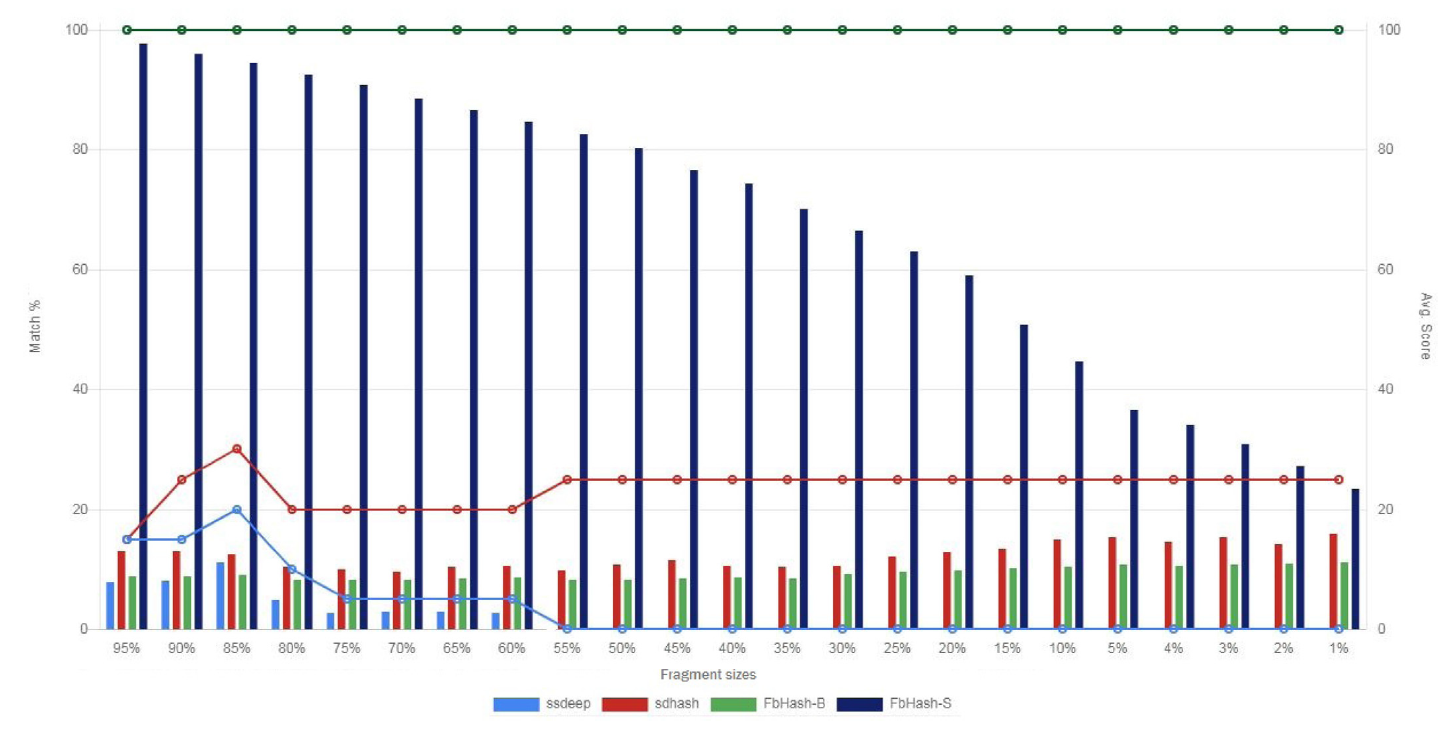
\includegraphics[width=1\columnwidth]{frag_det_docx.png}
\end{center}
\caption{\small{Rezultati testiranja avtorjev na datotekah tipa docx. Vir: \cite{fbhash}}}
\label{fig:fd-docx-rez}
\end{figure}

Tudi mera \texttt{F-score} na datotekah tipa docx pokaže, da je \texttt{FbHash-S} za njih najbolj primeren. Ta ima oceno 92\%, dočimer algoritmi \texttt{ssdeep}, \texttt{sdhash} in \texttt{FbHash-B} dosežejo 40\%, 41\% in 24\%.

\subsubsection{Korelacija skupnega dela datoteke}

Testi korelacije skupnega dela datoteke so bili narejeni na bazi podatkov, ki vsebujejo datoteke s skupnimi deli različnih velikosti. Te datoteke so tekstovne ter datoteke tipa docx iz \cite{zdataset}. 

Rezultati testov pokažejo, da se na tekstovnih datotekah \texttt{ssdeep} odreže najslabše in sicer z verjetnostjo $\geq 75\%$ zazna, da se datoteki ujemata, ko imata skupni del velikosti $\geq 30\%$, a ta verjetnost pri manjših delih hitro pade. \texttt{Sdhash} se bolje izkaže, saj zazna skupne dele, ki so veliki $\geq 3\%$ z verjetnostjo $\geq 93\%$. \texttt{FbHash} se izkaže najbolje, saj pade verjetnost, da zazna datoteki s skupnim delom pod $100\%$ šele, ko imata skupen del, ki je velikosti le $1\%$. Takrat je verjetnost $\geq 93\%$.

Tudi na datotekah tipa docx rezultati testov pokažejo, da se \texttt{ssdeep} odreže najslabše. Ta ima največjo verjetnost, ko imata datoteki skupen del velikosti 10\% in sicer 30\%. Drugi velikosti skupnega dela pa dajo verjetnost $\leq 20\%$. Boljše rezultate doseže \texttt{sdhash}, ki ugotovi ujemanje datotek z skupnim delom velikosti 5\% in 10\% z verjetnostjo 90\%. Zanimiv je rezultat funkcij \texttt{FbHash-B} in \texttt{FbHash-S}. Rezultat \texttt{FbHash-S} pokaže ujemanje 100\% dokler imata datoteki skupnega več kot 2\% in nato 90\%. \texttt{FbHash-B} pa ugotovi, da imata datoteki skupen del z verjetnostjo 100\% ko imata datoteki skupnega manj kot 40\%. Ko imata skupnega več ta verjetnost pade na 80\%.
\\
\section{Na\v{s}i eksperimenti}
Glavni cilj naših testov je bil ugotoviti, kateri izmed načinov določanja uteži dosega najboljše rezultate. V ta namen smo algoritma \texttt{FbHash-B} in \texttt{FbHash-S} implementirali~\cite{repo}, pripravili okolje za testiranje delovanja zgoščevalne funkcije ter preizkusili več načinov izračunavanja uteži.

\subsection{Testiranje algoritma}
Pri testiranju algoritma smo sledili postopku, ki so ga opisali avtorji dela \cite{fbhash}.

\subsubsection{Generiranje testnih primerov}
Algoritem smo testirali na prosto dostopni bazi datotek \cite{zdataset}. Iz baze smo uporabili 100 besedilnih ter html datotek.

Testne primere za algoritem smo generirali tako, da iz zbirke vzamemo dve različni datoteki in naključen blok prvega vstavimo na naključno mesto v drugi datoteki na tak način, da je znan delež druge datoteke sedaj enak delu prve datoteke. Tako dobimo par datotek z natančno znanim ujemanjem.

\subsubsection{Ocenjevanje delovanja algoritma}
Da so naši rezultati čimbolj primerljivi s temi, ki so jih objavili v članku \cite{fbhash}, smo tudi mi algoritem testirali na parih datotek z različnimi deleži ujemanja in opazovali dve vrednosti. Prva nam pove v kolikšnem deležu parov je algoritem odkril kakršnokoli ujemanje, druga pa predstavlja povprečno vrednost ujemanja, ki jo je algoritem izmeril. S tem lahko preverjamo kako majhne bloke besedila algoritem še prepozna in kako močna povezava obstaja med napovedano ter dejansko podobnostjo.

Tako kot v originalnem delu, smo se tudi mi odločili meriti vrednost F-score. Pri tem smo naključno generirali datoteke z različnimi merami ujemanja, med katerimi polovica datotek sploh ni imela nobenega ujemanja. Nato smo z algoritmom določili stopnjo ujemanja in opazovali, ali je ujemanje zaznal.

\section{Rezultati}
Testirali smo več različnih funkcij za izračun uteži delov datotek.

Najprej si oglejmo delovanje funkcije, ki jo predlagajo avtorji članka \cite{fbhash} in je bila prva opisana v poglavju \ref{utezivclanku}. Rezultati so predstavljeni na sliki \ref{fig:clanekUtezi}. Algoritem s to formulo za uteži je dosegel F-score 94\%, kar se ujema z vrednostjo, ki so jo dobili v članku.
\begin{figure}[htb]
\begin{center}
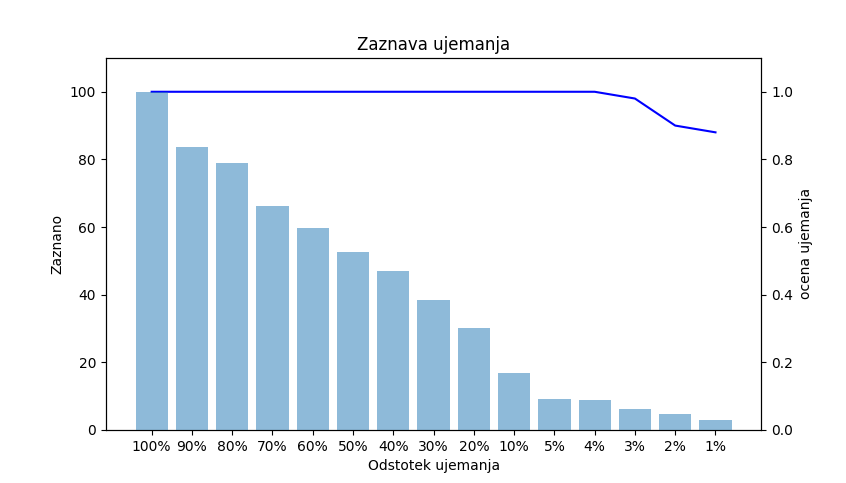
\includegraphics[width=1\columnwidth]{njihov_majhen.png}
\end{center}
\caption{\small{Rezultati testiranja z utežmi opisanimi v članku.}}
\label{fig:clanekUtezi}
\end{figure}

Rezultati, ki smo jih dobili se skladajo s tem, kar je predstavljeno v raziskavi v \cite{fbhash}. Vidimo lahko, da resnično ujemanje datotek ter izmerjena podobnost dobro sovpadata, vidimo pa tudi, da je algoritem v vseh primerih prepoznal delno ujemanje za vse dele datotek večje od 4\% datoteke.

Ker se nam formula za izračun uteži ne zdi smiselna, smo jo nekoliko spremenili v obliko, ki je prav tako opisana v poglavju \ref{utezivclanku}.

\begin{figure}[htb]
\begin{center}
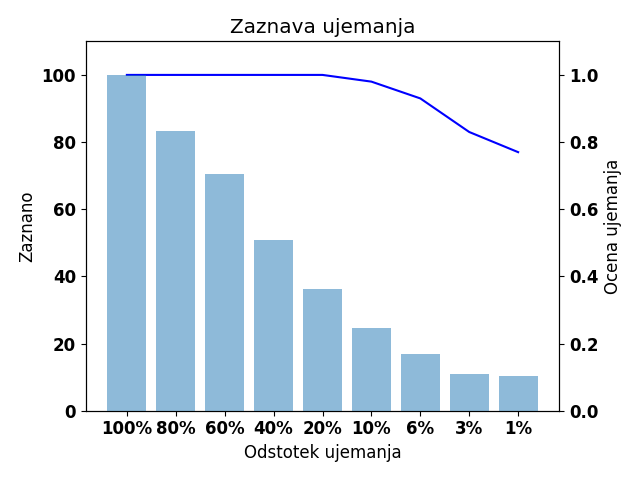
\includegraphics[width=1\columnwidth]{ch_tfidf_weight_majhna.png}
\end{center}
\caption{\small{Rezultati testiranja s prilagojenimi utežmi.}}
\label{fig:ch_tfidf}
\end{figure}

V tem primeru smo dosegli F-score 93\%, kar je zelo blizu prejšnjega rezultata.

Kot utež smo poskusili uporabiti tudi razmerje med frekvenco dela besedila in številom delov besedila. Tako smo ponovno dobili podobne rezultate (glej sliko \ref{fig:ch_freq}). Pri tem smo izmerili F-score 92\%.

\begin{figure}[htb]
\begin{center}
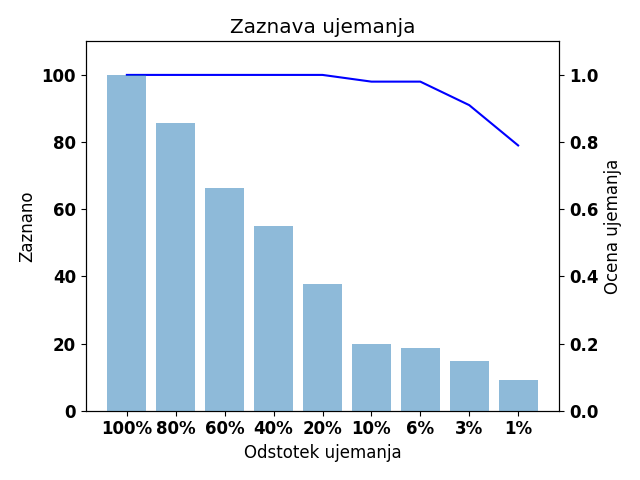
\includegraphics[width=1\columnwidth]{ch_freq_weight.png}
\end{center}
\caption{\small{Rezultati testiranja z razmerjem med frekvenco dela ter številom vseh delov}}
\label{fig:ch_freq}
\end{figure}

Pri teh testih smo opazili, da se rezultati pri različnih utežeh ne razlikujejo zelo veliko, zato smo poskusili tudi, kaj bi se zgodilo, če bi začetno analizo zbirke datotek izpustili in kot uteži uporabili konstantno vrednost (glej sliko \ref{fig:brezZbirke}). V tem primeru smo dosegli F-score vrednost 87\%. Pri tem smo ugotovili, da zaradi tega zaznava podobnosti datotek res deluje slabše, saj algoritem že pri 20\% ujemanju datotek v nekaterih primerih ujemanja ni prepoznal, vendar pa povezava med napovedano in resnično podobnostjo še vedno ostaja dovolj močna. Ta rezultat pomeni, da bi lahko predlagani algoritem uporabili za primerjavo datotek tudi v primerih, kjer nimamo velike zbirke gradiva na katerem lahko izračunamo uteži.

\begin{figure}[htb]
\begin{center}
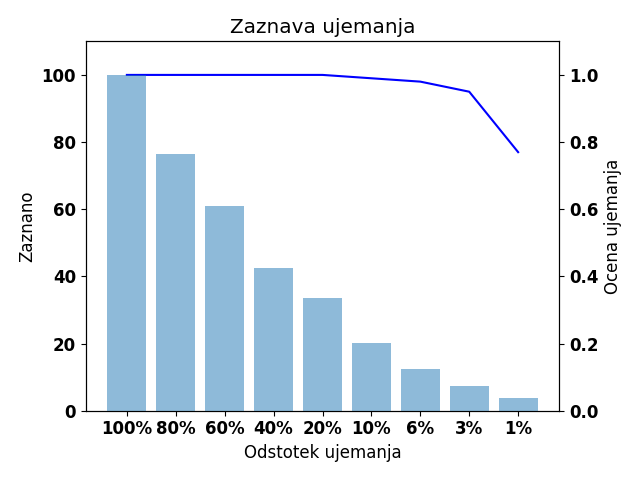
\includegraphics[width=1\columnwidth]{brez_courpusa.png}
\end{center}
\caption{\small{Rezultati testiranja brez uporabe zbirke besedil.}}
\label{fig:brezZbirke}
\end{figure}

\FloatBarrier
 
Vprašali smo se tudi, kaj bi se zgodilo v primeru, da bi namesto konstantnih uteži uporabili naključne vrednosti. V tem primeru so bili rezultati podobni tisti, kjer smo uporabili konstantno vrednost, F-score vrednost pa je dosegla 89\%.


\section{Zaklju\v{c}ek}
V delu smo opisali algoritem za detekcijo podobnih delov datotek \texttt{FbHash}. Algoritem smo implementirali z več različicami funkcij za uteženje posameznih delov datotek. Implementacijo smo testirali na istih množicah kot so jih uporabili avtorji algoritma. Naša implementacija je dosegla F-score 94\%, kar je enako kot v članku~\cite{fbhash}. Ugotovili smo, da je algoritem uporaben tudi z relativno majhno bazo datotek.
\\
\section{Zahvala}
%Mogoče zahvala avtorjem za narjeno delo al kej.
V tem delu smo se močno opirali na članek~\cite{fbhash}, zato se iskreno zahvaljujemo avtorjem članka za opravljeno delo in razvoj algoritma \texttt{FbHash}. Algoritem \texttt{FbHash} je pomemben prispevek digitalni forenziki.

\bibliographystyle{abbrv}
\bibliography{sigproc}  % sigproc.bib is the name of the Bibliography in this case
% You must have a proper ".bib" file
%  and remember to run:
% latex bibtex latex latex
% to resolve all references

%%\balancecolumns
%\appendix
%%Appendix A

\balancecolumns
\end{document}

% Now, we'll enter an unnumbered equation:
%\begin{displaymath}\sum_{i=0}^{\infty} x + 1\end{displaymath}
%and follow it with another numbered equation:
%\begin{equation}\sum_{i=0}^{\infty}x_i=\int_{0}^{\pi+2} f\end{equation}
%just to demonstrate \LaTeX's able handling of numbering.

%To set a wider table, which takes up the whole width of the page's live area, use the environment \textbf{table*} to enclose the table's contents 

%\begin{table*}
%\centering
%\caption{Some Typical Commands}
%\begin{tabular}{|c|c|l|} \hline
%Command&A Number&Comments\\ \hline
%\texttt{{\char'134}alignauthor} & 100& Author alignment\\ \hline
%\texttt{{\char'134}numberofauthors}& 200& Author enumeration\\ \hline
%\texttt{{\char'134}table}& 300 & For tables\\ \hline
%\texttt{{\char'134}table*}& 400& For wider tables\\ \hline\end{tabular}
%\end{table*}
% end the environment with {table*}, NOTE not {table}!

%\begin{figure}
%\centering
%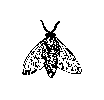
\epsfig{file=fly.eps}
%\caption{A sample black and white graphic (.eps format).}
%\end{figure}

%\begin{figure}
%\centering
%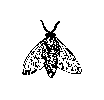
\epsfig{file=fly.eps, height=1in, width=1in}
%\caption{A sample black and white graphic (.eps format)
%that has been resized with the \texttt{epsfig} command.}
%\end{figure}

%As was the case with tables, you may want a figure that spans two columns. \textbf{figure*} to enclose the figure and its caption.

%\begin{figure*}
%\centering
%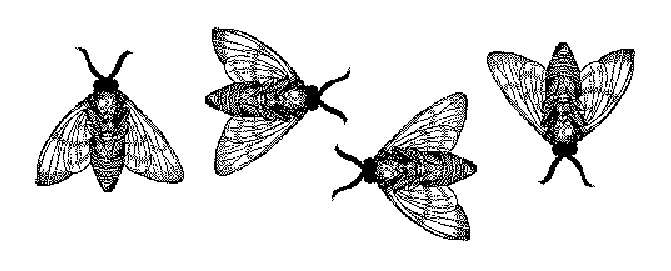
\epsfig{file=flies.eps}
%\caption{A sample black and white graphic (.eps format)
%that needs to span two columns of text.}
%\end{figure*}
%and don't forget to end the environment with
%{figure*}, not {figure}!

%This uses the \textbf{theorem} environment, created by
%the\linebreak\texttt{{\char'134}newtheorem} command:
%\newtheorem{theorem}{Theorem}
%\begin{theorem}
%Let $f$ be continuous on $[a,b]$.  If $G$ is
%an antiderivative for $f$ on $[a,b]$, then
%\begin{displaymath}\int^b_af(t)dt = G(b) - G(a).\end{displaymath}
%\end{theorem}

%The other uses the \textbf{definition} environment, created
%by the \texttt{{\char'134}newdef} command:
%\newdef{definition}{Definition}
%\begin{definition}
%If $z$ is irrational, then by $e^z$ we mean the
%unique number which has
%logarithm $z$: \begin{displaymath}{\log e^z = z}\end{displaymath}
%\end{definition}

%the \textbf{proof} environment.  Here
%is a example of its use:
%\begin{proof}
%Suppose on the contrary there exists a real number $L$ such that
%\begin{displaymath}
%\lim_{x\rightarrow\infty} \frac{f(x)}{g(x)} = L.
%\end{displaymath}
%Then
%\begin{displaymath}
%l=\lim_{x\rightarrow c} f(x)
%= \lim_{x\rightarrow c}
%\left[ g{x} \cdot \frac{f(x)}{g(x)} \right ]
%= \lim_{x\rightarrow c} g(x) \cdot \lim_{x\rightarrow c}
%\frac{f(x)}{g(x)} = 0\cdot L = 0,
%\end{displaymath}
%which contradicts our assumption that $l\neq 0$.
%\end{proof}